\chapter{Implementation}

In this chapter a reinforcement learning algorithm based on TD3 will be implemented that will be the framework for the reward function analysis in chapter 4.

\section{Environment and Interface}
Environment erklären - schnittstelle mit openAI gym - observation und action state erklären - einbau von algorithmus mit bild schnittstelle algorithmus zu environment 

\section{Algorithm Implementation}

\begin{figure} 
	\centering
	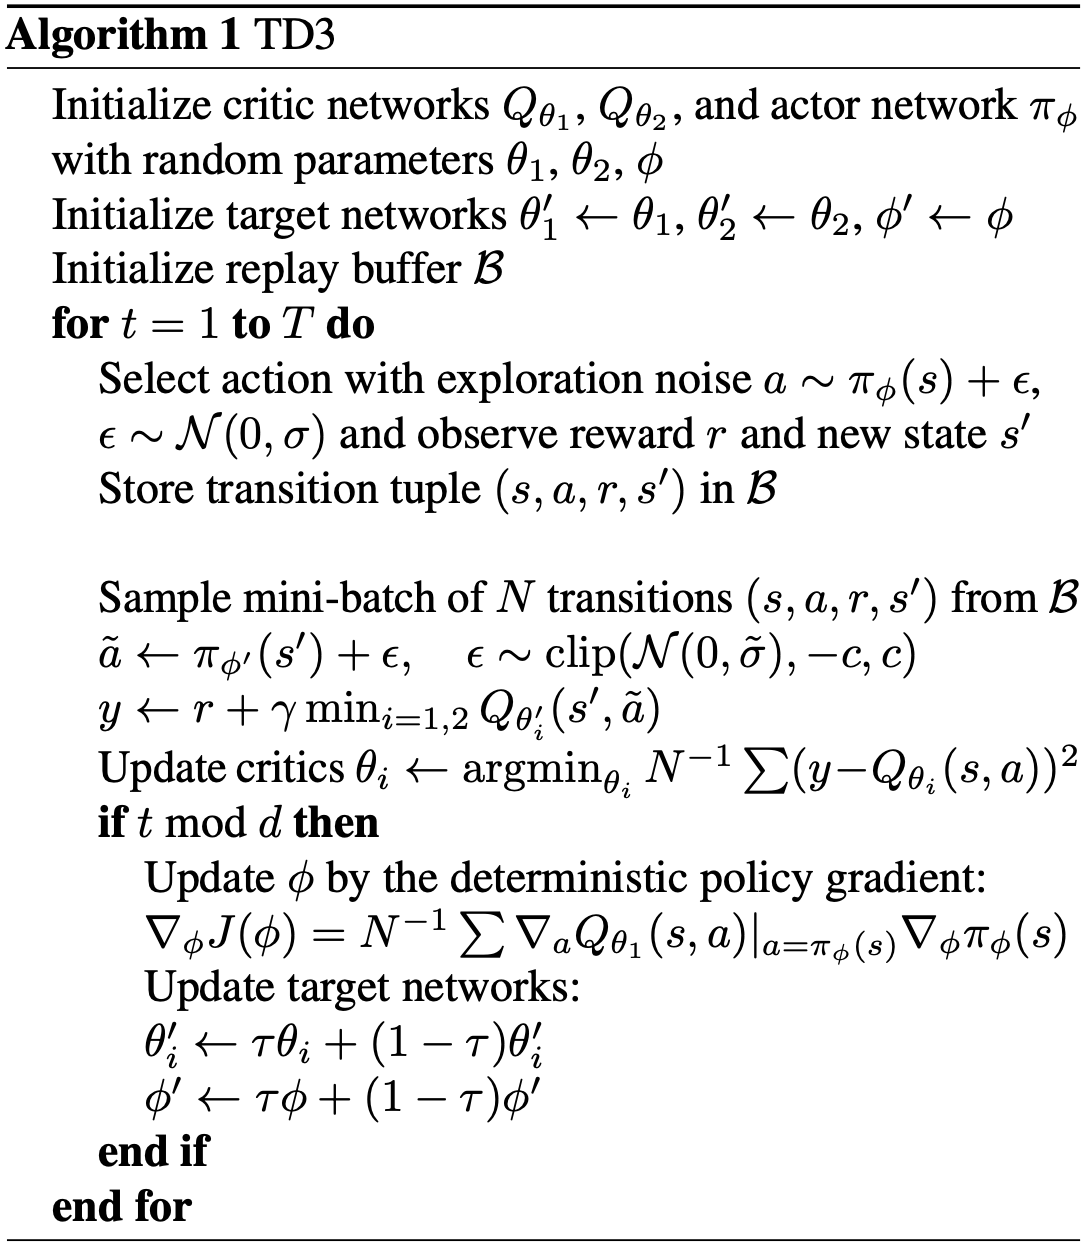
\includegraphics[scale=0.5]{img/Logo/TD3_pseudocode.png}
	\caption{Classification of machine learning}
	\label{fig:TD3_pseudo}
\end{figure}

Figure \ref{fig:TD3_pseudo} shows the rough structure of the twin delayed deep deterministic policy gradient (TD3) algorithm. It is an off policy actor critic method based the deep deterministic policy gradient algorithm \cite{lillicrap2015continuous}, with the enhancements of using Double Q-learning for the actors, delayed policy updates and target policy smoothing \cite{fujimoto2018}.

\subsection{Initializing actor and critic networks}
To initialize the actor and the critic, artificial neural networks are used.

\textbf{Artificial Neural Networks:}
An Artificial Neural Network (ANN) in simple terms is a biologically inspired
computational model, which consists of processing elements (called neurons), and
connections between them with coefficients (weights) bound to the connections.
These connections constitute the neuronal structure and attached to this structure are
training and recall algorithms. Neural networks are called the connectionist models
because of the connections found between the neurons
\subsection{Deep Q-Learning}
\subsection{Policy Gradient}

\subsection{Build Agent}
jo
\subsubsection{Actor and Critic}
actor critic networks and target networks with mathematical equations
and number of layers, nodes... 
\subsubsection{Replay Buffer and Gaussian Noise}
input layer states and actions, output layer with activation function...
initialization with random weights and 400, 300 nodes...
\subsection{Train Agent}
jo
\subsubsection{Loss Function}
\subsubsection{Network Update}
